%% ============================================================
% f2012_sichuan_sci_q14_cube.tex
%% 2012 四川卷（理科）第 14 题 正方体 ABCD-A1B1C1D1，M、N 分别为 CD、CC1 的中点
%% 来源 PDF：普通高考/2012/2012四川理.pdf 第 1 页（印面 771）第 3 栏
%% 坐标取自原页矢量层（bp），原点为图区左上角 (908.0,55.0)，y 向下；虚线照原页。
%% ============================================================
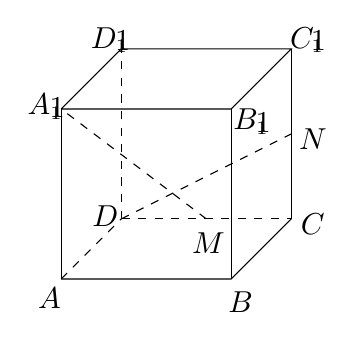
\begin{tikzpicture}[x=1bp,y=-1bp,
  every node/.style={inner sep=0,font=\fontsize{10.5pt}{12.6pt}\selectfont},
  line cap=butt, line join=miter]
  \draw[line width=0.398bp] (17.738,97.422) -- (78.945,97.422) -- (100.582,75.785);
  \draw[line width=0.398bp] (17.738,36.215) -- (78.945,36.215) -- (100.582,14.574) -- (39.375,14.574) -- (17.738,36.215);
  \draw[line width=0.398bp] (78.945,97.422) -- (78.945,36.211);
  \draw[line width=0.398bp] (100.586,75.785) -- (100.586,14.574);
  \draw[line width=0.398bp] (17.738,97.422) -- (17.738,36.211);
  \draw[line width=0.398bp, dash pattern=on 2.989bp off 2.989bp] (17.738,97.422) -- (39.375,75.785);
  \draw[line width=0.398bp, dash pattern=on 2.989bp off 2.989bp] (39.375,75.785) -- (100.586,75.785);
  \draw[line width=0.398bp, dash pattern=on 2.989bp off 2.989bp] (39.375,75.785) -- (39.375,14.574);
  \draw[line width=0.398bp, dash pattern=on 2.989bp off 2.989bp] (69.98,75.785) -- (17.738,36.215);
  \draw[line width=0.398bp, dash pattern=on 2.989bp off 2.989bp] (39.375,75.785) -- (100.586,45.18);
  \node[anchor=base west] at (28.22,14.4) {$D_1$};
  \node[anchor=base west] at (36.91,15.29) {$1$};
  \node[anchor=base west] at (99.91,14.4) {$C_1$};
  \node[anchor=base west] at (107.41,15.29) {$1$};
  \node[anchor=base west] at (5.47,38.31) {$A_1$};
  \node[anchor=base west] at (13.35,39.2) {$1$};
  \node[anchor=base west] at (79.55,43.65) {$B_1$};
  \node[anchor=base west] at (87.51,44.54) {$1$};
  \node[anchor=base west] at (103.15,50.74) {$N$};
  \node[anchor=base west] at (28.8,78.69) {$D$};
  \node[anchor=base west] at (103.81,81.35) {$C$};
  \node[anchor=base west] at (64.68,88.33) {$M$};
  \node[anchor=base west] at (9.22,107.93) {$A$};
  \node[anchor=base west] at (77.74,109.44) {$B$};
\end{tikzpicture}
